\documentclass[a2paper, 12pt]{article}
\usepackage[font={huge, bf}]{caption}
\usepackage{fontspec}
\setmainfont{Arial}
\usepackage{subcaption}
\usepackage{graphicx}
\usepackage{tikz}
\usepackage{tikzsymbols}
\usetikzlibrary{calc,patterns,shapes.geometric}
\usepackage{float}
\usepackage{pdflscape}
\usepackage{geometry}
\geometry{landscape, margin=2cm}
\captionsetup[subfigure]{justification=justified,singlelinecheck=false}
\pagestyle{empty}

\def\centerarc[#1](#2)(#3:#4:#5){\draw[#1] ($(#2)+({#5*cos(#3)},{#5*sin(#3)})$) arc (#3:#4:#5);}

\begin{document}
	\vspace*{\fill}
	\begin{figure}[!htbp]
		\centering
		\begin{subfigure}[b]{0.48\textwidth}
			\caption{Figure 1}
			\centering
			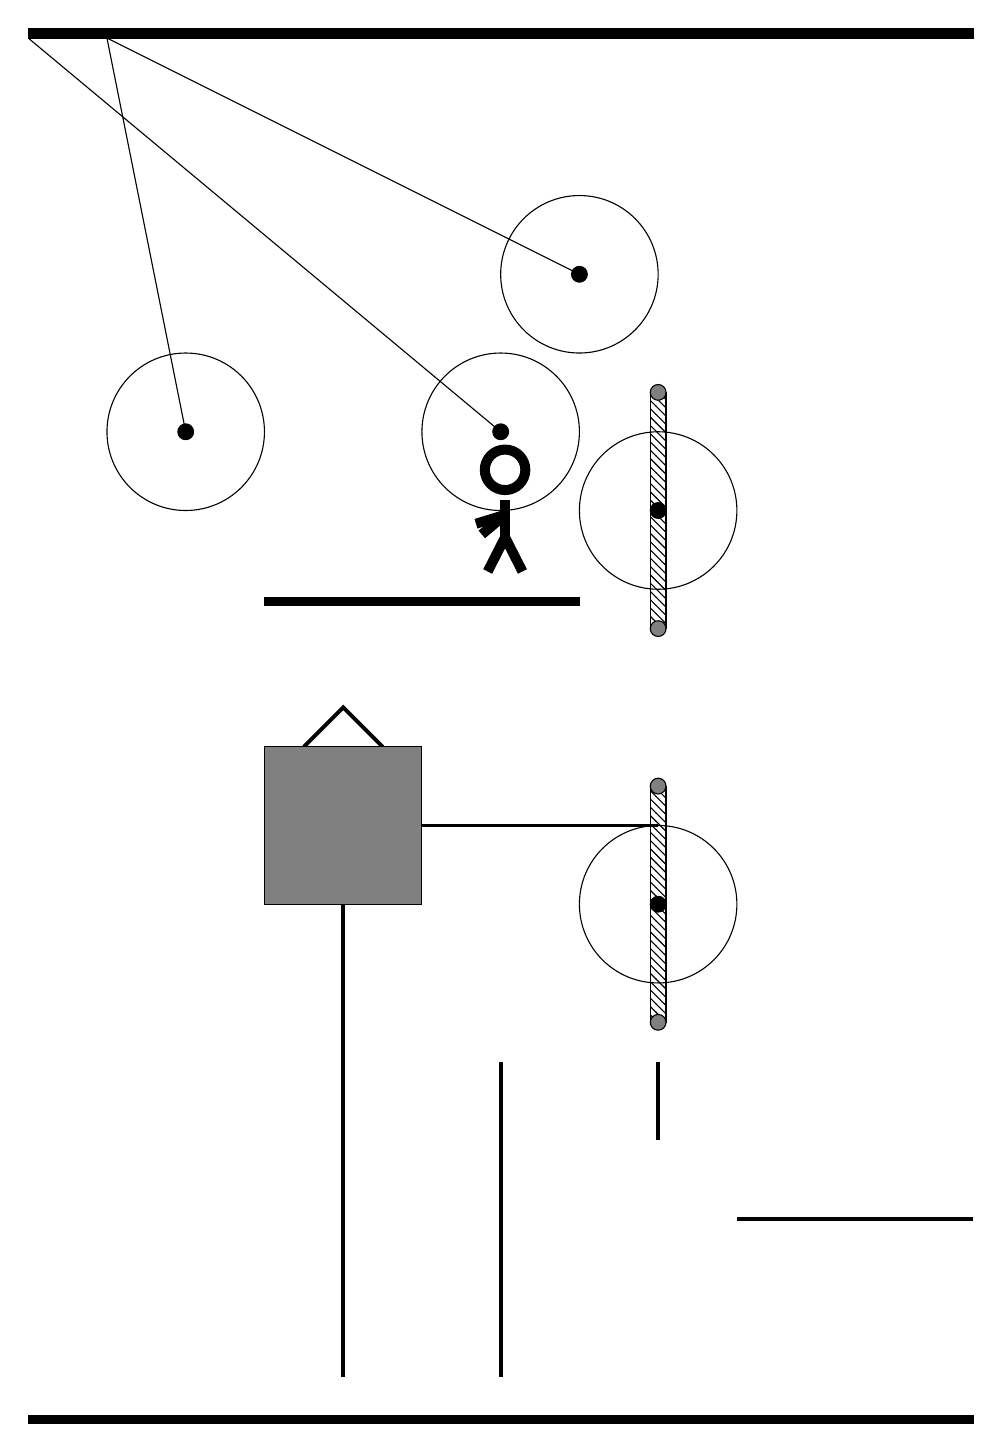
\begin{tikzpicture}
				\draw[fill=black] (-2, 14) rectangle (10, 14.125);
				
				\draw (4,9) circle (1);
				\draw[fill=black] (4,9) circle (0.1);
				\draw (-2,14.0) -- (4,9);
				
				\draw (5,11) circle (1);
				\draw[fill=black] (5,11) circle (0.1);
				\draw (-1,14.0) -- (5,11);
				
				\draw (0,9) circle (1);
				\draw[fill=black] (0,9) circle (0.1);
				\draw (-1,14.0) -- (0,9);
				
				\draw (6,8) circle (1);
				\draw[fill=black] (6,8) circle (0.1);
				\draw[pattern=north west lines, pattern color=black] (5.9,9.5) rectangle (6.1,6.5);
				\draw[fill=black!50] (6,9.5) circle (0.1);
				\draw[fill=black!50] (6,6.5) circle (0.1);
				
				\draw (6,3) circle (1);
				\draw[fill=black] (6,3) circle (0.1);
				\draw[pattern=north west lines, pattern color=black] (5.9,4.5) rectangle (6.1,1.5);
				\draw[fill=black!50] (6,4.5) circle (0.1);
				\draw[fill=black!50] (6,1.5) circle (0.1);
				
				\draw[line width=0.5mm](1.5,5) --  (2,5.5) -- (2.5,5);
				\draw[fill=black!50] (1, 5) rectangle (3, 3);
				
				\draw[line width = 0.5mm] (3,4) -- (6,4);
				\centerarc[line width = 0.5mm](3,3)(90:180:1);
				\draw[line width = 0.5mm] (2,3) -- (2,-3);
				\centerarc[line width = 0.5mm](3,-3)(180:360:1);
				\draw[line width = 0.5mm] (4,-3) -- (4,1);
				\centerarc[line width = 0.5mm](5,1)(0:180:1);
				\draw[line width = 0.5mm] (6,1) -- (6,0);
				\centerarc[line width = 0.5mm](7,0)(180:270:1);
				\draw[line width = 0.5mm] (7,-1) -- (10,-1);
				
				\node at (4, 8) {\scriptsize \Strichmaxerl[10][40][-163]};
				\draw[fill=black] (1, 6.9) rectangle (5, 6.8);
				
				\draw[fill=black] (-2, -3.5) rectangle (10, -3.6);
			\end{tikzpicture}
		\end{subfigure}
		\hfill
		\begin{subfigure}[b]{0.48\textwidth}
			\caption{Figure 2}
			\centering
			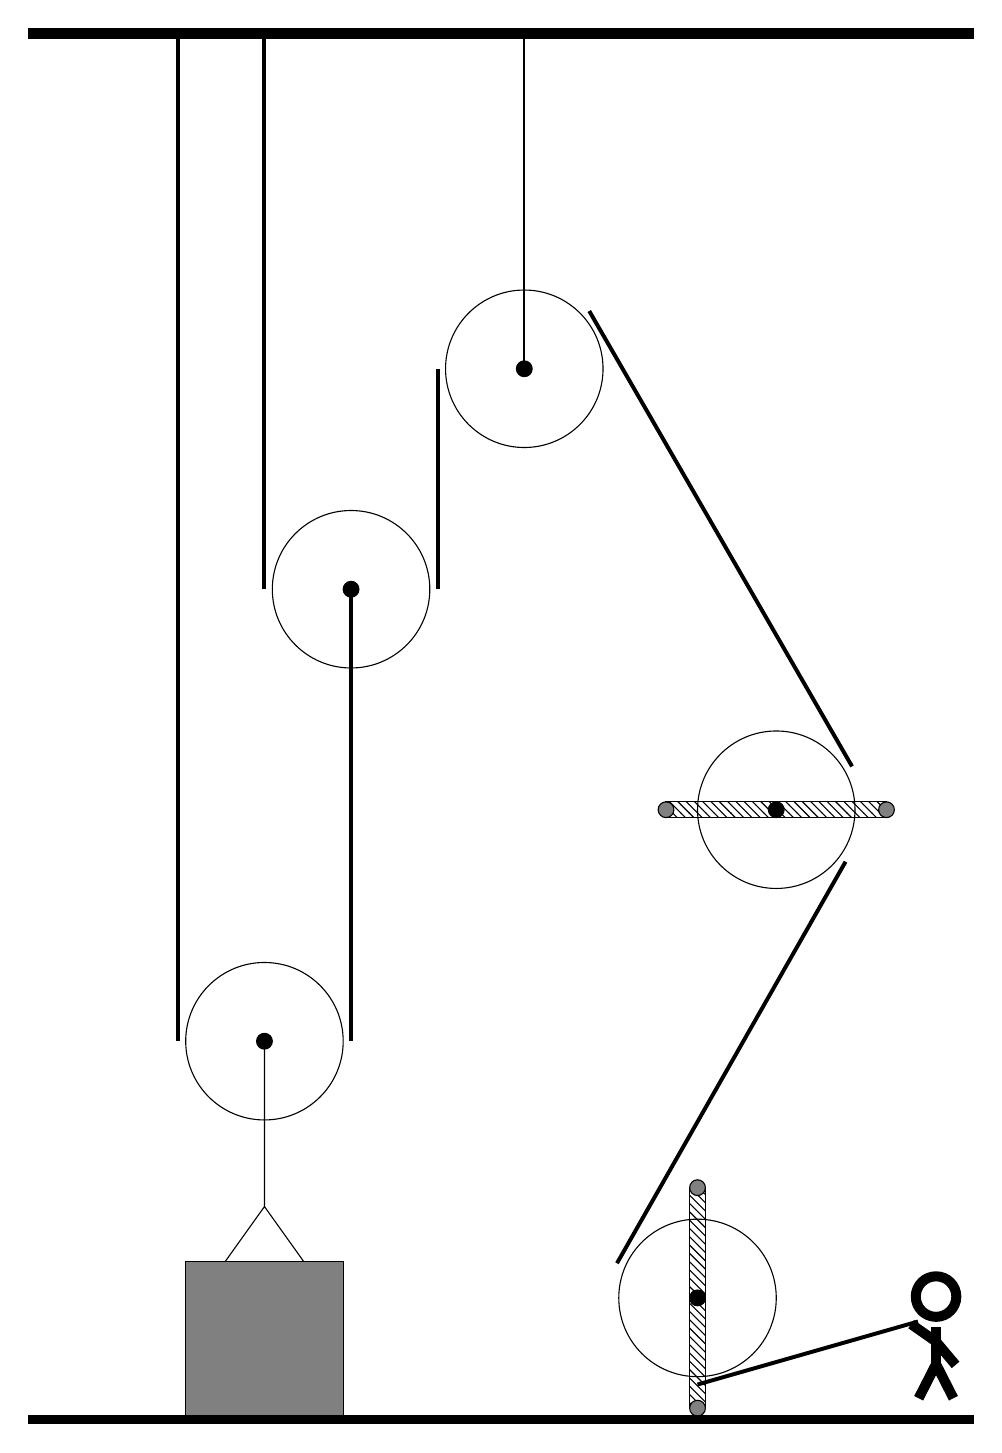
\begin{tikzpicture}
				\draw[fill=black] (-2, 14) rectangle (10, 14.125);
				
				\draw (1, 1.26) circle (1);
				\draw[fill=black] (1, 1.26) circle (0.1);
				
				\draw (2.1, 7.0) circle (1);
				\draw[fill=black] (2.1, 7.0) circle (0.1);
				
				\draw (4.3, 9.8) circle (1);
				\draw[fill=black] (4.3, 9.8) circle (0.1);
				\draw[thick] (4.3, 9.8) -- (4.3, 14);
				
				\draw (6.5, -2) circle (1);
				\draw[fill=black] (6.5, -2) circle (0.1);
				\draw[pattern=north west lines, pattern color=black] (6.4, -0.6) rectangle (6.6, -3.4);
				\draw[fill=black!50] (6.5, -0.6) circle (0.1);
				\draw[fill=black!50] (6.5, -3.4) circle (0.1);
				
				\draw (7.5, 4.2) circle (1);
				\draw[fill=black] (7.5, 4.2) circle (0.1);
				\draw[pattern=north west lines, pattern color=black] (6.1, 4.3) rectangle (8.9, 4.1);
				\draw[fill=black!50] (6.1, 4.2) circle (0.1);
				\draw[fill=black!50] (8.9, 4.2) circle (0.1);
				
				\draw (1, 1.26) -- (1, -0.84) -- (0.5, -1.54) -- (1.5, -1.54) -- (1, -0.84);
				\draw[fill=black!50] (0, -1.54) rectangle (2, -3.54);
				
				\draw[line width=0.5mm] (-0.1, 14) -- (-0.1, 1.26);
				\centerarc[line width=0.5mm](1, 1.26)(180:360:1.1);
				\draw[line width=0.5mm](2.1, 1.26) -- (2.1, 7.0);
				\draw[line width=0.5mm] (1.0, 14) -- (1.0, 7.0);
				\centerarc[line width=0.5mm](2.1, 7.0)(180:360:1.1);
				\draw[line width=0.5mm](3.2, 7.0) -- (3.2, 9.8);
				\centerarc[line width=0.5mm](4.3, 9.8)(35:180:1.1);
				\draw[line width=0.5mm] (5.125, 10.5333) -- (8.4625, 4.75);
				\centerarc[line width=0.5mm](7.5, 4.2)(215:135:-1.1);
				\draw[line width=0.5mm](8.38, 3.54) -- (5.477, -1.56);
				\centerarc[line width=0.5mm](6.5, -2)(-30:100:-1.1);
				\draw[line width=0.5mm](6.5, -3.1) -- (9.3, -2.3);
				
				\node at (9.5, -2.5) {\scriptsize \Strichmaxerl[10][-35][-50]};
				
				\draw[fill=black] (-2, -3.5) rectangle (10, -3.6);
			\end{tikzpicture}
		\end{subfigure}
	\end{figure}
		\vspace*{\fill}
\end{document}